\documentclass[12pt]{article}
\usepackage{amsmath}
\usepackage{amssymb}
\usepackage{graphicx}
\usepackage{comment}

\begin{document}

\title{\textbf{REQUIREMENTS ANALYSIS DOCUMENT }}
\maketitle

\begin{center}
\title{\textbf{Software Design COMS3009}}
\maketitle 
\end{center}
\begin{center}
\title{\textbf{FindMeTutor Android Application}}
\maketitle 
\end{center}

\begin{center}
Proposed idea by:\\
Shaneel James-718840
\\Jadon Manilal-815050
\\Jared Naidoo - 719238
\\Krupa Prag - 782681
\\Nivek Ranjith - 802119
\end{center}

\newpage

%TABLE OF CONTENTS
\tableofcontents
\newpage
%INTRODUCTION
\section{INTRODUCTION}
\subsubsection{Purpose of the system}
\begin{flushleft}
The purpose of the FindMeTutor application is to provide a convenient means for tutors and students who are looking for tutors to be able to connect within a particular tertiary institute.
\end{flushleft}
\subsubsection{Scope of the system}
\begin{flushleft}
Our team, working on the FindMeTutor application, envisions a successful product to be an Android Application which will be at a students's disposal in order to improve their grades and achieve their academic dreams. With limited resources a  stringent budget and capped time, we aim to execute this task in an economical fashion.\\
This goal will be achieved by making use of agile methodology. We will be able to set short term targets to achieve deliverables within sprints, with a long term goal being to present the FindMeTutor Android Application. 
\end{flushleft}
\subsubsection{Objective and success criteria of the project}
\begin{flushleft}
The FindMeTutor Android application will be seen as successful if it facilitates a platform on which tutors and students can meet. We have great hope that the result of this would mean better results obtained by the students, and a manner in which tutors can generate some income and gain some job experience. 
\end{flushleft}
\subsubsection{Definitions, acronyms, and abbreviations}
1. App - abbreviation for application. \\
2. Application - is a piece of software \\
3. Android - is a mobile operating system developed by Google. \\
4. OS - abbreviation for operating system.\\
5. Operating system - is a collection of software that communicates with hardware and allows other programs to run on it. It comprises  of system software, or the fundamental files your computer needs to boot up and function.\\
6. Boot up - Processes started when computer is turned on\\
7. Java - is a high-level programming language\\
8. UI - abbreviation for User interface\\
9. User interface - is the means in which a person controls a software application or hardware device.
10. ID - abbreviation for identity\\
11.User ID - the idenity that uniquely identifies someone on a computer system.\\
12. Sign in - when asked to enter username and password information. A sign in/ login is a combination of information that authenticates a user's identity. \\
 

\subsubsection{References}
1. http://techterms.com/definition (2016-08-08)
%\subsubsection{Overview}
%dummy text

%CURRENT SYSTEM
\section{CURRENT SYSTEM}
\subsubsection{Overview}
\begin{flushleft}
Currently, there are many students in search of tutors to help them with particular courses with which they require some support, as well as fellow students or tutors who are available to tutor particular courses of study. However, the problem that is faced on hand is that either pool (students and tutors) are struggling to find each other. 
\end{flushleft}

%PROPOSED SYSTEM
\section{PROPOSED SYSTEM}
\subsection{Overview}
\begin{flushleft}
FindMeTutor app will be a platform through which students and tutors can meet in order to resolve the current situation. 
\end{flushleft}
\begin{flushleft}
FindMeTutor app will facilitate the following two registration categories: 

\begin{flushleft}
1.Student looking for tutors – they are able to  register on the app with merely some personal details (demographic data, faculty registration details, security answer and password).\\
2. Tutor - those who would like to tutor can register on the app by simply filling in some details with respect to the fields of study they are particularly comfortable to tutor.\\
\end{flushleft}
\end{flushleft}
\subsection{Functional requirements - "Shall lists"}

Describes the high-level functionality of the system\\

\begin{comment}
3.2.1 The database has the ability to store data captured of the users of the application (student and tutors data).More specifically, the database will be able to accept numeric data entry and will store the courses under the University of Wthe Witwatersrand's School of Compute science and Applied mathematics undergraduate topics which will be displayed in the drop-down menu when students and tutors will be required to select the courses respectively to which they are enrolled in or able to tutor. \\
3.2.2 The app will provide an effective means through which tutors and students can communicate. The messenger facility will facilitate communication between students and tutors - when students request a tutor, the tutor and student will be able to use this facility to arrange a convenient time, place and tuition fee for the tutor service. \\
3.2.3 Request appropriate tutors for students who send a request on the app for a tutor eligible to tutuor a specific course (aid to pair up appropriate tutors and students).\\
3.2.4 In the light of security, the database shall be able store a corresponding password for each user of the application, which will allow for each users account to be protected, as each user's user ID and entered password will be compared to that of which was entered into the database at sign-up, hence the system restricting access to authorized users. \\
3.2.5 FindMeTutor Android application will be able to be utilised on any Android OS of (some version), which is able easily accessible,as many students can download this application for use on their smartphones and/or tablets which shall makes the application easily accessible. 
\end{comment}

{
\centering
\begin{tabular}{| l | p{10cm}| l |}
			\hline			
			\textbf{Requirement} & \textbf{Functional Requirement} & \textbf{Use Case}
			
			\\ \hline RQ1.1 & The system shall allow a student to register  & UC-CS \\ \hline 
			RQ1.2 & The system shall allow a student to update their account & UC-US \\ \hline  
			RQ1.3 & The system shall allow a student to view their account details  & UC-VS \\ \hline 
			RQ1.4 & The system shall allow a student to mark their account as deleted & UC-DS  \\ \hline 
			RQ2.1 & The system shall allow a tutor to register & UC-CT \\ \hline
			RQ2.2 & The system shall allow a tutor to update their account  & UC-UT \\ \hline
			RQ2.3 & The system shall allow a tutor to view their account details & UC-VT \\ \hline
			RQ2.4 & The system shall allow a tutor to mark their account as deleted & UC-DT \\ \hline  
			
			RQ3.1 & The system shall allow a administrator to update a student account & UC-US \\ \hline  
			RQ3.2 & The system shall allow a administrator to view a student account details  & UC-VS \\ \hline 
			RQ3.3 & The system shall allow a administrator to mark a student as deleted & UC-DS  \\ \hline 
			RQ3.4 & The system shall allow a administrator to update a tutor account  & UC-UT \\ \hline
			RQ3.5 & The system shall allow a administrator to view a tutor account details & UC-VT \\ \hline
			RQ3.6 & The system shall allow a administrator to mark a tutor account as deleted & UC-DT \\ \hline			
			
\end{tabular}
}

\subsection{Non-functional requirements}{
Describes the user-level requirements that are not directly related to the functionality. \\
\\\textbf{3.3.1 Usability}\\ 
The application will be user friendly as it will be pitched as an Android application which is supported by multiple devices (smartphones and tablets) that has Android as an OS. This will allow for the application to be easily accessible to students and tutors as majority of the students have access to these devices. 
\\\textbf{3.3.2 Reliability}\\
The probability that the system will be able to process work correctly and completely without being aborted.\\
In the case of system failure, the damage that could be caused could be such where the personalised accounts of the application user will lose their preference choices of subjects selected on sign-up. 
\\\textbf{3.3.3 Performance}\\
The response time between the UI and the server will be(??). The expected volume of data (??). The expected volume of user activity will peak at the end of each academic term within the tertiary institute when examinations/tests will be approaching, while on a regular basis the application will be utilised when students who feel the need to get assistance immediately when they encounter a topic they require assistance in. 
\\\textbf{3.3.4 Supportability}\\
\textbf{3.3.5 Implementation}\\
Our team has implemented the agile methodology in order to obtain our final goal of building the FindMeTutor application. For each sprint we will set targets of what we would like to achieve, with the objective of using these milestones to be building blocks towards our final goal. 
\\\textbf{3.3.6 Interface}\\
The UI will be made in Android studio. The set up will be simple and neat. The app will be used by students who will be using the app in order to search for a tutor which is suitable to tutor, hence, with this intention, to prevent furthering the overwhelmed feeling, the app will not be clutered and simple to use. The 'user-friendly' experience provided by the UI, will allow the user to interact with the app in a natural and intuitive way. \\
Each user's hope page will be customized to the particular topics in which they are enrolled in or signed up to tutor, with respect to whether they are students or tutors. \\
\textbf{3.3.7 Packaging}\\
\textbf{3.3.8 Legal}\\
}
\subsection{System models}
\subsubsection{Scenario}
\begin{flushleft}
For instance, there is a student - Joe Soap - who is currently doing his  3rd year of study in computer science.  Joe would like to generate some income from tutoring first and second year mathematics modules. However, Joe is also looking for a 3rd year Mathematics tutor to help him with some of his mathematics courses. We also know that the student, Mary Smith, is a first year astronomy student who is looking for a mathematics tutor. The FindMeTutor app will be ideal to resolve the problems faced in this particular scenario. Joe will register on the application as a student and as a tutor, on registering, he will select what he is capable and willing to tutor - first and second year mathematics. On the other hand, we will have Mary register as a student. Mary will then be able to search for the course she needs assistance in, for example – Calculus I; any tutors who have uploaded material on this particular topic (Calculus I) will come up. Mary may find these resources useful, but if Mary does not get the assistance she requires from the material available, and would like to seek a personal tutor, Mary will click the 'Request tutor' button and this will send a request to all those who have registered to tutor Calculus I. Joe Soap will be part of the list of tutors approached. Joe accepts the request. Mary is notified of this and is now able to communicate with Joe to make further arrangements of time of meeting, venue and also to flag him of what sections she needs assistance in. On the other hand, Joe requires an 'Emergency lesson' – this is a last minute lesson before his test which is scheduled to take place in a day's time. Tutors eligible to tutor Joe's course will be sent an 'Urgent request'. A tutor that accepts this request will communicate with Joe through the messaging facility which is made available. If the only possible means of having a lesson before the test is to Skype each other, then the tutor and Joe will be redirected to a skype page which will facilitate this conference.
\end{flushleft}


\subsubsection{Use cases models}
\textbf{Use cases}	\\		
			Create Student		UC-CS
			\\Update Student 	UC-US
			\\View Student      UC-VS
			\\Archive Student	UC-DS
			\\Create Tutor		UC-CT
			\\Update Tutor		UC-UT
			\\View Tutor			UC-VT
			\\Archive Tutor		UC-DT
			\\			
		
		
		{
		\centering
		
		\begin{tabular}{| l | l| }
			\hline\multicolumn{2}{|c|}{ \textbf{Use Case UC-CS: Create Student}} \\ \hline
			Related Requirements: & RQ1.1 \\ \hline
			Initiating actor: & Student \\ \hline
			Actor goal: & To register on FindMeTutor\\ \hline
			Participating Actors: & External Database System\\ \hline
			Preconditions: & N/A\\ \hline
			Postconditions: & Student is created\\ \hline
			\multicolumn{2}{|l|}{Flow of activities:}\\ \hline
			\multicolumn{2}{|p{15cm}|}{1. Student indicates sign up}\\
			\multicolumn{2}{|p{15cm}|}{2. System displays student sign up form}\\
			\multicolumn{2}{|p{15cm}|}{3. Student enters demographic data, faculty registration details, security answer and password}	\\		
			\multicolumn{2}{|p{15cm}|}{4. System sends demographic data, faculty registration details, security answer and password to external database system}\\
			\multicolumn{2}{|l|}{5. Student is created}	
			\\ \hline		
		\end{tabular}
		
		\begin{tabular}{| l | p{10cm}| }
			\hline\multicolumn{2}{|c|}{ \textbf{Use Case UC-US: Update Student}} \\ \hline
			Related Requirements: & RQ1.2, RQ3.1 \\ \hline
			Initiating actor: & Student or Administrator \\ \hline
			Actor goal: & To update student demographic data, faculty registration details, security answer or password\\ \hline
			Participating Actors: & External Database System\\ \hline
			Preconditions: & Student exists\\ \hline
			Postconditions: & Student is updated\\ \hline
			\multicolumn{2}{|l|}{Flow of activities:}\\ \hline
			\multicolumn{2}{|p{15cm}|}{1. Student/Administrator requests to update Student}\\
			\multicolumn{2}{|p{15cm}|}{2. System displays form to update Student}\\
			\multicolumn{2}{|p{15cm}|}{3. Student/Administrator enters demographic data, faculty registration details or security answer}	\\		
			\multicolumn{2}{|p{15cm}|}{4. System sends demographic data, faculty registration details, security answer or password to external database system}\\
			\multicolumn{2}{|l|}{5. Student is updated}	
			\\ \hline		
		\end{tabular}
		
		\begin{tabular}{| l | l| }
		
			\hline\multicolumn{2}{|c|}{ \textbf{Use Case UC-CT: Create Tutor}} \\ \hline
			Related Requirements: & RQ2.1 \\ \hline
			Initiating actor: & Tutor \\ \hline
			Actor goal: & To register on FindMeTutor\\ \hline
			Participating Actors: & External Database System\\ \hline
			Preconditions: & N/A\\ \hline
			Postconditions: & Tutor is created\\ \hline
			\multicolumn{2}{|l|}{Flow of activities:}\\ \hline
			\multicolumn{2}{|p{15cm}|}{1. Tutor indicates sign up}\\
			\multicolumn{2}{|p{15cm}|}{2. System displays tutor sign up form}\\
			\multicolumn{2}{|p{15cm}|}{3. Tutor enters demographic data, courses tutored, security answer and password}	\\		
			\multicolumn{2}{|p{15cm}|}{4. System sends demographic data, courses tutored details, security answer and to external database system}\\
			\multicolumn{2}{|l|}{5. Tutor is created}	
			\\ \hline		
		\end{tabular}
		
		\begin{tabular}{| l | p{10cm}| }
			\hline\multicolumn{2}{|c|}{ \textbf{Use Case UC-UT: Update Tutor}} \\ \hline
			Related Requirements: & RQ2.2, RQ3.4 \\ \hline
			Initiating actor: & Tutor or Administrator \\ \hline
			Actor goal: & To update Tutor demographic data, courses tutored, security answer or password\\ \hline
			Participating Actors: & External Database System\\ \hline
			Preconditions: Tutor exists\\ \hline
			Postconditions: & Tutor is updated\\ \hline
			\multicolumn{2}{|l|}{Flow of activities:}\\ \hline
			\multicolumn{2}{|p{15cm}|}{1. Tutor/Administrator requests to update Tutor}\\
			\multicolumn{2}{|p{15cm}|}{2. System displays form to update Tutor}\\
			\multicolumn{2}{|p{15cm}|}{3. Tutor/Administrator enters demographic data, faculty registration details or security answer}	\\		
			\multicolumn{2}{|p{15cm}|}{4. System sends demographic data, faculty registration details, security answer or password to external database system}\\
			\multicolumn{2}{|l|}{5. Tutor is updated}	
			\\ \hline		
		\end{tabular}

		\begin{tabular}{| l | p{10cm}| }
			\hline\multicolumn{2}{|c|}{ \textbf{Use Case UC-DS: Archive Student}} \\ \hline
			Related Requirements: & RQ1.4, RQ3.3 \\ \hline
			Initiating actor: & Student or Administrator \\ \hline
			Actor goal: & To delete Student\\ \hline
			Participating Actors: & External Database System\\ \hline
			Preconditions: Student exists\\ \hline
			Postconditions: & Student is Archived\\ \hline
			\multicolumn{2}{|l|}{Flow of activities:}\\ \hline
			\multicolumn{2}{|p{15cm}|}{1. Student/Administrator requests to delete Student}\\
			\multicolumn{2}{|p{15cm}|}{2. System displays confirmation message}\\
			\multicolumn{2}{|p{15cm}|}{3. Student/Administrator enters confirmation}	\\		
			\multicolumn{2}{|p{15cm}|}{4. System sends archive Student signal to external database system}\\
			\multicolumn{2}{|l|}{5. Student is archived}	
			\\ \hline		
		\end{tabular}
		
		\begin{tabular}{| l | p{10cm}| }
			\hline\multicolumn{2}{|c|}{ \textbf{Use Case UC-DT: Archive Tutor}} \\ \hline
			Related Requirements: & RQ2.4, RQ3.6 \\ \hline
			Initiating actor: & Tutor or Administrator \\ \hline
			Actor goal: & To delete Tutor\\ \hline
			Participating Actors: & External Database System\\ \hline
			Preconditions: Tutor exists\\ \hline
			Postconditions: & Tutor is Archived\\ \hline
			\multicolumn{2}{|l|}{Flow of activities:}\\ \hline
			\multicolumn{2}{|p{15cm}|}{1. Tutor/Administrator requests to delete Tutor}\\
			\multicolumn{2}{|p{15cm}|}{2. System displays confirmation message}\\
			\multicolumn{2}{|p{15cm}|}{3. Tutor/Administrator enters confirmation}	\\		
			\multicolumn{2}{|p{15cm}|}{4. System sends archive Tutor signal to external database system}\\
			\multicolumn{2}{|l|}{5. Tutor is archived}	
			\\ \hline		
		\end{tabular}
		
		\begin{tabular}{| l | p{10cm}| }
			\hline\multicolumn{2}{|c|}{ \textbf{Use Case UC-VT: View Tutor}} \\ \hline
			Related Requirements: & RQ2.3, RQ3.5 \\ \hline
			Initiating actor: & Tutor or Administrator \\ \hline
			Actor goal: & To view Tutor\\ \hline
			Participating Actors: & External Database System\\ \hline
			Preconditions: Tutor exists\\ \hline
			Postconditions: & Tutor is viewed\\ \hline
			\multicolumn{2}{|l|}{Flow of activities:}\\ \hline
			\multicolumn{2}{|p{15cm}|}{1. Tutor/Administrator requests to view Tutor}\\
			\multicolumn{2}{|p{15cm}|}{2. System displays Tutor}\\
			\multicolumn{2}{|l|}{3. Tutor is viewed}	
			\\ \hline		
		\end{tabular}	
		
		\begin{tabular}{| l | p{10cm}| }
			\hline\multicolumn{2}{|c|}{ \textbf{Use Case UC-VS: View Student}} \\ \hline
			Related Requirements: & RQ1.3, RQ3.2 \\ \hline
			Initiating actor: & Student or Administrator \\ \hline
			Actor goal: & To view Student\\ \hline
			Participating Actors: & External Database System\\ \hline
			Preconditions: Student exists\\ \hline
			Postconditions: & Student is viewed\\ \hline
			\multicolumn{2}{|l|}{Flow of activities:}\\ \hline
			\multicolumn{2}{|p{15cm}|}{1. Student/Administrator requests to view Student}\\
			\multicolumn{2}{|p{15cm}|}{2. System displays Student}\\
			\multicolumn{2}{|l|}{3. Student is viewed}	
			\\ \hline		
		\end{tabular}	
		
		}
	\newpage	
\subsubsection{Use case diagrams}
{
		

		\centering
		Use case diagram: Create Student	\\
		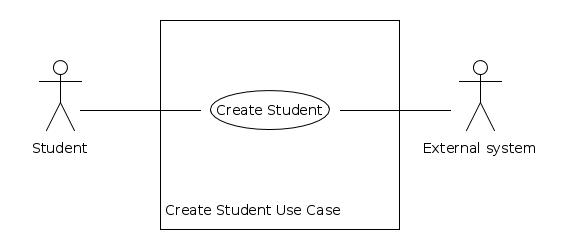
\includegraphics[width=140mm]{/home/shaneel/Documents/FindMeTutor/Use_Cases/Create_Student.jpg}
		Use case diagram: Update Student \\
		\centering
		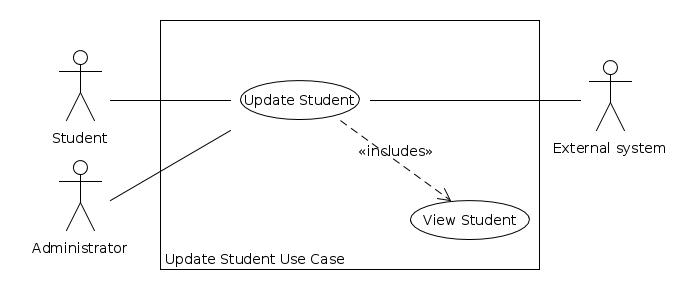
\includegraphics[width=140mm]{/home/shaneel/Documents/FindMeTutor/Use_Cases/Update_Student.jpg}
		Use case diagram: View Student \\
		\centering
		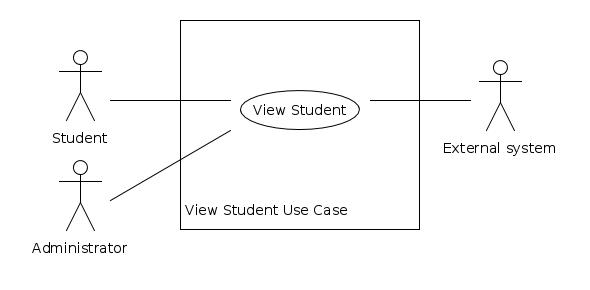
\includegraphics[width=140mm]{/home/shaneel/Documents/FindMeTutor/Use_Cases/View_Student.jpg}
		Use case diagram: Archive Student \\
		\centering
		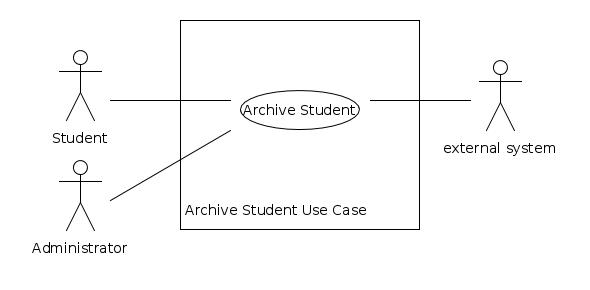
\includegraphics[width=140mm]{/home/shaneel/Documents/FindMeTutor/Use_Cases/Archive_Student.jpg}
		Use case diagram: Create Tutor\\
		\centering
		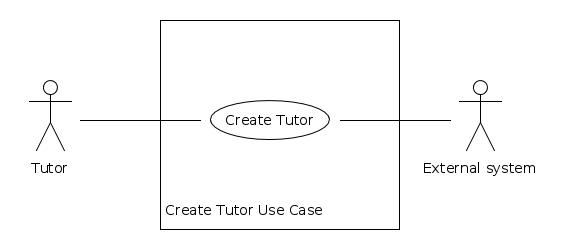
\includegraphics[width=140mm]{/home/shaneel/Documents/FindMeTutor/Use_Cases/Create_Tutor.jpg}
		Use case diagram: Update Tutor \\
		\centering
		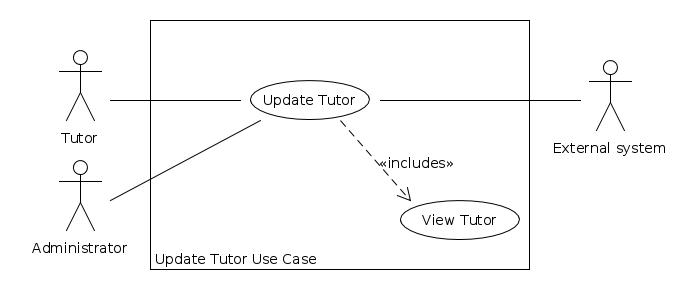
\includegraphics[width=140mm]{/home/shaneel/Documents/FindMeTutor/Use_Cases/Update_Tutor.jpg}
		Use case diagram: View Tutor \\
		\centering
		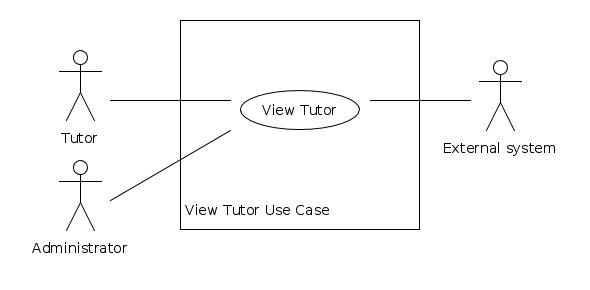
\includegraphics[width=140mm]{/home/shaneel/Documents/FindMeTutor/Use_Cases/View_Tutor.jpg}
		Use case diagram: Archive Tutor \\
		\centering
		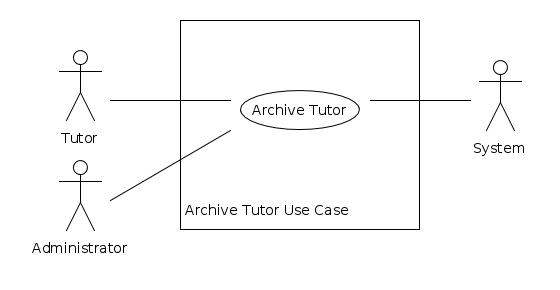
\includegraphics[width=140mm]{/home/shaneel/Documents/FindMeTutor/Use_Cases/Archive_Tutor.jpg}
		
		
}

		
\newpage
\subsubsection{Analysis object model}

\subsubsection{Dynamic model}
A dynamic model represents the behaviour of an object over time. It is used where the object's behaviour is best described as a set of states that occur in a defined sequence. The components of the dynamic model are:\\
 	States. The purchase order (PO) is modelled as passing through a set of states. The operations that can be performed on the PO are dependent on the state it is in. For example, information cannot be entered after it has reached the approved state.\\
	State transitions. When purchase order data entry has been completed it transitions from the entering PO state to the pending approval state. State transitions are modelled as being instantaneous.\\
	Events. Events trigger state transitions. For example, the order mailed event triggers a state transition from the approved to the placed state.\\
	Actions. Actions occur on state transitions. For example, on a goods received event the action of notify purchaser is performed. Actions are modelled as instantaneous occurrences (contrast with activities).\\
	Activities. An activity is performed while an object is in a specific state. For example, while in the entering PO state data is entered into the PO. Activities are modelled as occurring over a period of time (contrast with actions).\\
	(Will add diagram)\\
\subsubsection{User interface navigational paths and screen mock-ups} 

\subsubsection{Operational requirements}
Operational requirements describe the non-business characteristics of an application.\\
3.5.1 Amazon Web Server - Web server to host the database\\ 
3.5.2 Android studio to design UI\\
3.5.3 GitHub to facilitate the build of the project among team members\\
3.5.4 MySql which is the database management system used to house and control the database.\\
%GLOSSARY
%\section{GLOSSARY}

%\section{REFERENCES}

\end{document}





